\subsection{Diseño de datos}
La estructura de datos inicial se basa en la tabla de usuarios predeterminada de \textbf{Supabase}, la cual incluye los campos mínimos necesarios para la autenticación de usuarios (destacamos id, email, contraseñas, fecha de creación y entre otos). Por otro lado, se ha creado una tabla \textbf{profiles} para almacenar información adicional de los usuarios (para este primer incremento solo se ha incluido el nombre de usuario, descripción y fecha de creación). Las tablas de \textbf{usuarios} y \textbf{profiles} están directamente relacionadas entre sí a través del \textbf{id} de la tabla de autenticación, tal y como podemos observar en \figref{fig:diagrama_datos_i1}.

\begin{figure}[H]
    \centering
    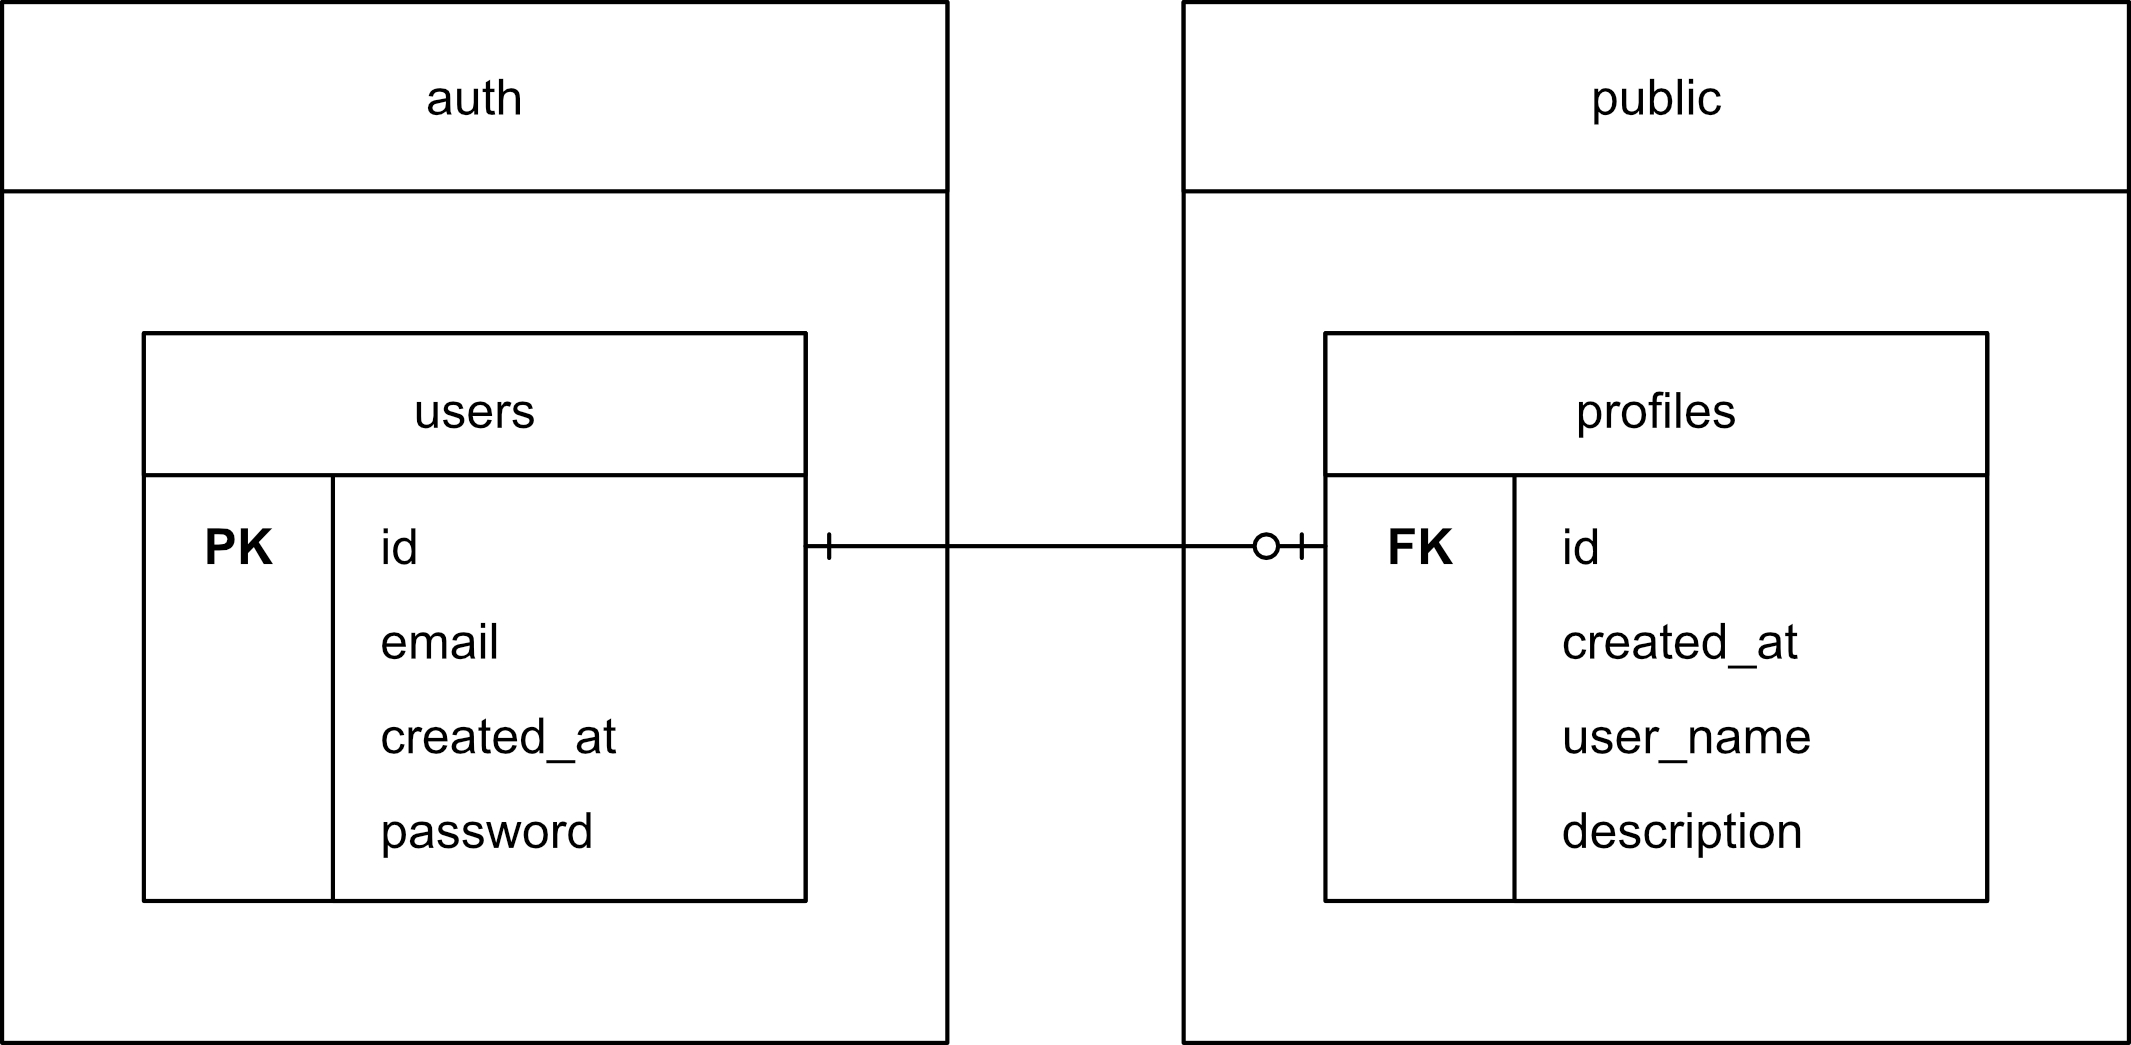
\includegraphics[width=0.8\textwidth]{Ilustraciones/desarrollo/incremento1/diagrama_datos_i1.jpg}
    \caption{Diagrama de estructura de datos de los perfiles de usuario}\label{fig:diagrama_datos_i1}
\end{figure}
